\documentclass[12pt, a4paper]{article}

% ─── Packages ────────────────────────────────────────────────────────────────
\usepackage[a4paper, margin=2.5cm]{geometry}
\usepackage{parskip}          % space between paragraphs instead of indent
\usepackage{titlesec}         % section heading style
\usepackage{titletoc}         % TOC style
\usepackage{fancyhdr}         % headers / footers
\usepackage{hyperref}         % clickable TOC links
\usepackage{listings}         % code blocks
\usepackage{xcolor}           % colours for code
\usepackage{booktabs}         % nicer tables
\usepackage{array}            % column type control
\usepackage{tabularx}         % auto-width tables
\usepackage{amsmath}          % math
\usepackage{graphicx}         % images (if needed later)
\usepackage{microtype}        % better text justification
\usepackage{enumitem}         % list spacing control
\usepackage{mdframed}         % framed note boxes
\usepackage{caption}

% ─── Colours ─────────────────────────────────────────────────────────────────
\definecolor{darkblue}{HTML}{1a2744}
\definecolor{midblue}{HTML}{2c4a8c}
\definecolor{codebg}{HTML}{f4f4f4}
\definecolor{codeborder}{HTML}{cccccc}
\definecolor{codestring}{HTML}{008000}
\definecolor{codecomment}{HTML}{888888}
\definecolor{codekeyword}{HTML}{0000cc}
\definecolor{notebg}{HTML}{e8f5ed}
\definecolor{noteborder}{HTML}{1f7a4a}
\definecolor{formulabg}{HTML}{fce4d6}
\definecolor{formulaborder}{HTML}{c55a11}

% ─── Hyperref setup ──────────────────────────────────────────────────────────
\hypersetup{
  colorlinks = true,
  linkcolor  = midblue,
  urlcolor   = midblue,
  pdftitle   = {Stereo Vision Face Depth Estimation},
  pdfauthor  = {Akash Dhande},
}

% ─── Section heading style ───────────────────────────────────────────────────
\titleformat{\section}
  {\large\bfseries\color{darkblue}}
  {\thesection.}{0.6em}{}
  [\vspace{-4pt}\color{midblue}\rule{\linewidth}{0.6pt}]

\titleformat{\subsection}
  {\normalsize\bfseries\color{midblue}}
  {\thesubsection.}{0.5em}{}

\titleformat{\subsubsection}
  {\normalsize\bfseries}
  {\thesubsubsection.}{0.5em}{}

\titlespacing{\section}{0pt}{18pt}{8pt}
\titlespacing{\subsection}{0pt}{12pt}{5pt}
\titlespacing{\subsubsection}{0pt}{10pt}{4pt}

% ─── Header / footer ─────────────────────────────────────────────────────────
\pagestyle{fancy}
\fancyhf{}
\fancyhead[L]{\small\color{darkblue}\textbf{Stereo Vision Face Depth Estimation}}
\fancyhead[R]{\small\color{darkblue}Intel RealSense D455F}
\fancyfoot[C]{\small\thepage}
\renewcommand{\headrulewidth}{0.4pt}

% ─── Code listing style ──────────────────────────────────────────────────────
\lstset{
  language         = Python,
  backgroundcolor  = \color{codebg},
  basicstyle       = \ttfamily\small,
  keywordstyle     = \color{codekeyword}\bfseries,
  stringstyle      = \color{codestring},
  commentstyle     = \color{codecomment}\itshape,
  numbers          = left,
  numberstyle      = \tiny\color{gray},
  numbersep        = 8pt,
  frame            = single,
  rulecolor        = \color{codeborder},
  breaklines       = true,
  tabsize          = 4,
  showstringspaces = false,
  captionpos       = b,
}

% For inline code
\newcommand{\code}[1]{\texttt{\small#1}}

% ─── Note / formula boxes ────────────────────────────────────────────────────
\newmdenv[
  backgroundcolor = notebg,
  linecolor       = noteborder,
  linewidth       = 1pt,
  leftmargin      = 0pt,
  rightmargin     = 0pt,
  innerleftmargin = 10pt,
  innerrightmargin= 10pt,
  innertopmargin  = 6pt,
  innerbottommargin=6pt,
  skipabove       = 8pt,
  skipbelow       = 8pt,
]{notebox}

\newmdenv[
  backgroundcolor = formulabg,
  linecolor       = formulaborder,
  linewidth       = 1pt,
  leftmargin      = 0pt,
  rightmargin     = 0pt,
  innerleftmargin = 12pt,
  innerrightmargin= 12pt,
  innertopmargin  = 8pt,
  innerbottommargin=8pt,
  skipabove       = 8pt,
  skipbelow       = 8pt,
]{formulabox}

% ─── TOC style ───────────────────────────────────────────────────────────────
\setcounter{tocdepth}{2}

% ─── List spacing ────────────────────────────────────────────────────────────
\setlist[itemize]{itemsep=3pt, topsep=4pt}
\setlist[enumerate]{itemsep=3pt, topsep=4pt}

% ─────────────────────────────────────────────────────────────────────────────
\begin{document}

% ─── Title page ──────────────────────────────────────────────────────────────
\begin{titlepage}
  \centering
  \vspace*{3cm}
  {\LARGE\bfseries\color{darkblue} Stereo Vision Face Depth Estimation\par}
  \vspace{0.5cm}
  {\large Using the Intel RealSense D455F Dual-IR Camera\par}
  \vspace{0.3cm}
  {\normalsize\itshape A technical report on stereo vision, disparity estimation,\\
  and real-time face depth measurement\par}
  \vspace{0.8cm}
  {\large Akash Dhande\par}
  \vspace{0.2cm}
  {\normalsize CS 5097 --- Mixed Reality\par}
  {\normalsize Prof.\ Ryan Bockmon\par}
  \vspace{1.0cm}
  \rule{0.6\linewidth}{0.4pt}\\[0.4cm]
  \begin{tabular}{ll}
    \textbf{Camera}       & Intel RealSense D455F (Dual IR Stereo) \\[4pt]
    \textbf{Methods}      & Hardware Depth \textbullet\ OpenCV SGBM \textbullet\ Custom SAD \\[4pt]
    \textbf{Face detector}& Google BlazeFace (MediaPipe TFLite) \\[4pt]
    \textbf{Date}         & \today \\
  \end{tabular}\\[0.4cm]
  \rule{0.6\linewidth}{0.4pt}
\end{titlepage}

% ─── Table of contents ───────────────────────────────────────────────────────
\tableofcontents
\newpage

% ─────────────────────────────────────────────────────────────────────────────
\section{Introduction and Project Overview}
% ─────────────────────────────────────────────────────────────────────────────

This project implements a real-time face depth estimation system using an
\textbf{Intel RealSense D455F} depth camera. The system captures four
synchronized streams simultaneously --- an RGB colour stream, a hardware depth
stream, and two infrared (IR) streams --- and uses them to detect human faces
and compute the distance of each detected face from the camera using three
independent methods.

The core motivation is to compare three fundamentally different depth estimation
strategies operating on the same input data in real time:

\begin{itemize}
  \item \textbf{Hardware Depth (Intel ASIC):} The D455F's onboard stereo
        processor computes depth maps at the hardware level using Intel's
        proprietary, FPGA-accelerated algorithm. This provides the highest
        quality reference depth map.

  \item \textbf{Semi-Global Block Matching (SGBM):} A classical computer vision
        algorithm implemented in OpenCV. It uses dynamic programming along
        multiple directions to produce smooth, high-quality disparity maps from
        the raw IR stereo pair.

  \item \textbf{Sum of Absolute Differences (SAD) Block Matching:} A custom
        NumPy implementation of the simplest stereo matching algorithm. It
        performs a brute-force search over all possible disparities for every
        pixel, optimised using the integral image (cumulative sum) technique.
\end{itemize}

All three methods are visualised simultaneously in a real-time
\textbf{six-panel grid}, with face bounding boxes and depth measurements
overlaid on each panel. This allows direct visual comparison of the quality,
noise characteristics, and accuracy of each approach.

% ─────────────────────────────────────────────────────────────────────────────
\section{Background Concepts}
% ─────────────────────────────────────────────────────────────────────────────

\subsection{The Pinhole Camera Model}

A camera is modelled mathematically as a \textbf{pinhole camera}: a 3D world
point $P = (X, Y, Z)$ is projected onto the 2D image plane at pixel coordinates
$(u, v)$ through the camera's focal point. The projection is governed by the
\textbf{intrinsic matrix} $K$:

\begin{equation}
  \begin{bmatrix} u \\ v \\ 1 \end{bmatrix}
  = K \cdot \begin{bmatrix} X/Z \\ Y/Z \\ 1 \end{bmatrix},
  \qquad
  K = \begin{bmatrix} f_x & 0 & c_x \\ 0 & f_y & c_y \\ 0 & 0 & 1 \end{bmatrix}
\end{equation}

\begin{center}
\begin{tabular}{lll}
  \toprule
  \textbf{Parameter} & \textbf{Meaning} & \textbf{Typical value (D455F, 640$\times$480)} \\
  \midrule
  $f_x$ & Focal length in $x$ (pixels) & $\approx$ 380--420 px \\
  $f_y$ & Focal length in $y$ (pixels) & $\approx$ 380--420 px \\
  $c_x$ & Principal point $x$          & $\approx$ 320 px \\
  $c_y$ & Principal point $y$          & $\approx$ 240 px \\
  \bottomrule
\end{tabular}
\end{center}

\subsection{Stereo Vision Fundamentals}

Stereo vision mimics human binocular depth perception. Two cameras, separated
by a known \textbf{baseline distance} $B$, observe the same scene from slightly
different viewpoints. Because the cameras are displaced horizontally, a 3D point
in the scene projects to \emph{different horizontal positions} in the two image
planes. This horizontal shift is called \textbf{disparity}.

\begin{figure}[h]
\centering
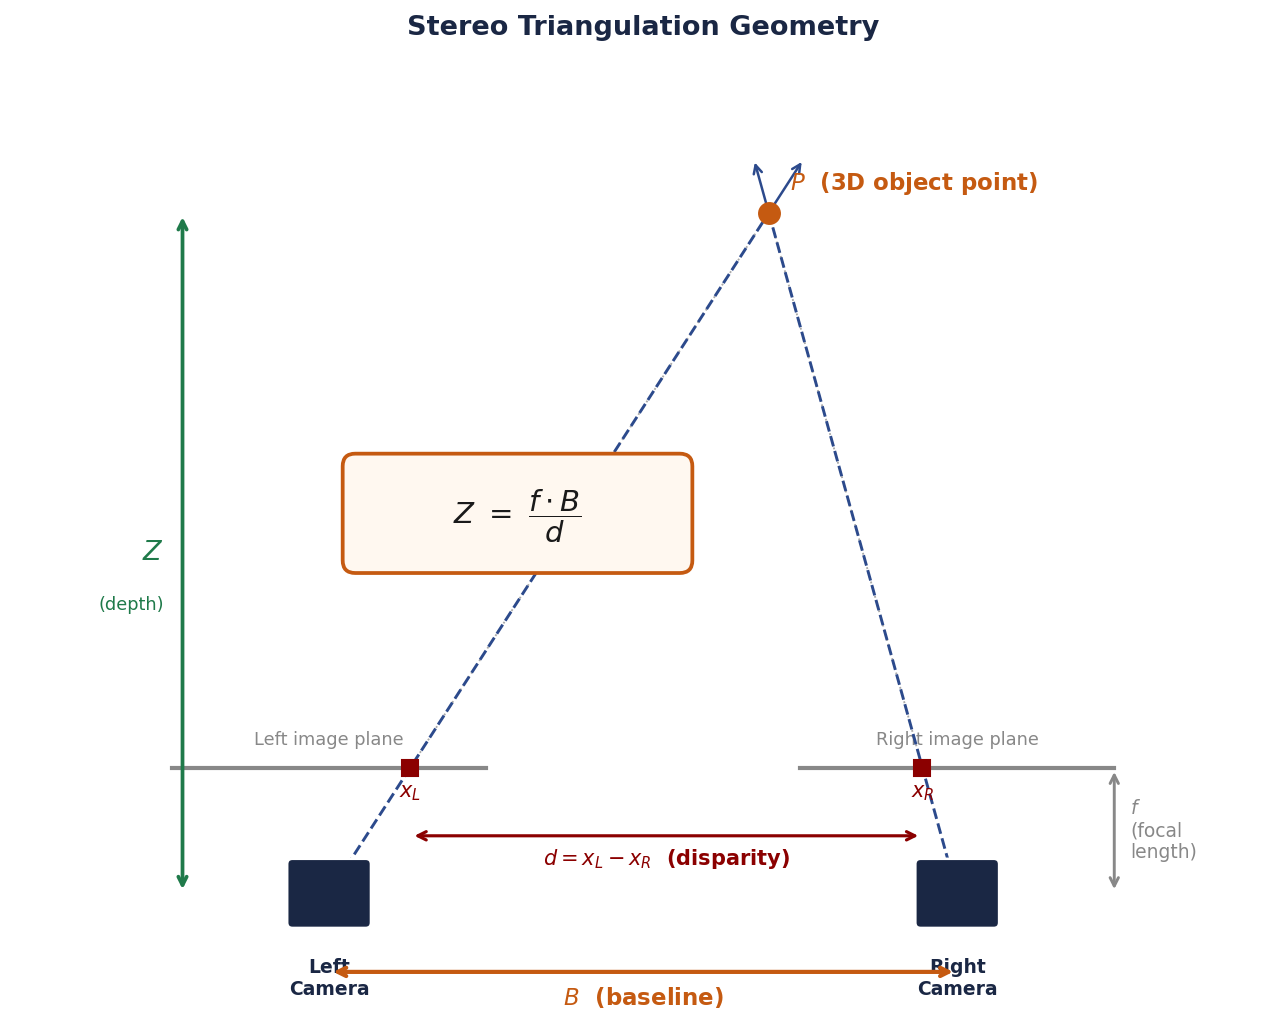
\includegraphics[width=0.85\linewidth]{stereo_triangulation.png}
\caption{Stereo triangulation geometry. The same 3D point $P$ projects to
different horizontal positions $x_L$ and $x_R$ in the left and right image
planes. The horizontal shift $d = x_L - x_R$ is the disparity, and depth is
recovered as $Z = f \cdot B \,/\, d$.}
\end{figure}

\subsection{Disparity and Depth Relationship}

For a \textbf{rectified stereo pair} (where both cameras share the same
horizontal scan lines), the relationship between disparity and depth is given by
the stereo triangulation formula:

\begin{formulabox}
\begin{equation}
  Z = \frac{f_x \cdot B}{d}
\end{equation}
where $Z$ = depth (metres), $f_x$ = focal length in pixels, $B$ = baseline in
metres, $d$ = disparity in pixels.
\end{formulabox}

\textbf{Key observation:} Depth is \emph{inversely proportional} to disparity.
Closer objects have larger disparity; distant objects have smaller disparity. At
zero disparity (infinity), depth is undefined --- this is why stereo cameras
have a maximum useful range.

This formula is used identically for both the SGBM and SAD approaches in this
project:

\begin{lstlisting}[caption={Disparity to depth conversion (live\_stream.py)}]
# fx and baseline extracted once at startup from camera intrinsics/extrinsics
depth_metres = (fx * baseline) / disparity_pixels
\end{lstlisting}

\subsection{Stereo Rectification}

In a real stereo camera, the two cameras are never perfectly aligned.
\textbf{Rectification} applies homographic transformations to both images so
that corresponding points lie on the \emph{same horizontal scan line}. After
rectification, stereo matching reduces from a 2D search to a 1D search along
rows, dramatically reducing computation.

\begin{notebox}
\textbf{Note:} The IR streams from the D455F are pre-rectified by the camera
firmware. The SGBM and SAD algorithms in this project can therefore directly
search along horizontal rows without any additional rectification step.
\end{notebox}

\subsection{Infrared Imaging for Stereo}

Visible-light stereo matching struggles in textureless or uniformly lit regions
because block matching requires local image texture to find correspondences.
The D455F addresses this with an \textbf{IR dot projector} that floods the scene
with a random dot pattern in the near-infrared spectrum ($\approx$850~nm),
invisible to the human eye. This creates artificial texture on featureless
surfaces (walls, clothing), dramatically improving stereo matching reliability.

The two IR cameras capture this textured scene as 8-bit grayscale images
(Y8 format, single channel). These IR images are the direct input to both the
SGBM and SAD algorithms.

\subsection{Block Matching for Stereo}

Block matching is the fundamental operation underlying most local stereo
matching algorithms. For each pixel $(y, x)$ in the left image:

\begin{enumerate}
  \item Extract a small $W \times W$ patch (block) centred at $(y, x)$.
  \item Search along the same horizontal row in the right image for disparities
        $0$ to $D$.
  \item Compute a \textbf{similarity metric} between the left block and each
        right-image candidate block.
  \item Assign the disparity $d^*$ that minimises the dissimilarity metric.
\end{enumerate}

Common metrics include SAD (Sum of Absolute Differences), SSD (Sum of Squared
Differences), and NCC (Normalized Cross-Correlation). This project uses
\textbf{SAD} for the custom implementation. Block size $W$ controls a key
trade-off: larger blocks are more robust to noise but lose precision near depth
discontinuities; smaller blocks preserve edges but are noisier.

% ─────────────────────────────────────────────────────────────────────────────
\section{Intel RealSense D455F Camera}
% ─────────────────────────────────────────────────────────────────────────────

\subsection{Hardware Architecture}

The Intel RealSense D455F is a factory-calibrated stereo depth camera designed
for depth sensing up to $\sim$6~metres. It integrates multiple sensors on a
single board:

\begin{center}
\begin{tabular}{lll}
  \toprule
  \textbf{Component} & \textbf{Description} & \textbf{Role in this project} \\
  \midrule
  IR Left Camera   & Global shutter, Y8 format   & Left image for SGBM \& SAD \\
  IR Right Camera  & Global shutter, Y8 format   & Right image for SGBM \& SAD \\
  RGB Camera       & Colour, BGR8 format          & Face detection input \\
  IR Dot Projector & 850~nm near-IR pattern       & Adds texture for stereo matching \\
  Stereo ASIC      & Intel Vision Processor D4    & Hardware depth map (Z16) \\
  IMU              & Accelerometer + Gyroscope    & Not used in this project \\
  \bottomrule
\end{tabular}
\end{center}

The physical layout from left to right on the camera bar is:
IR Left Camera --- IR Dot Projector --- RGB Camera --- IR Right Camera.
The baseline between the two IR cameras is approximately \textbf{95~mm}.

\subsection{Sensor Specifications}

\begin{center}
\begin{tabular}{ll}
  \toprule
  \textbf{Parameter} & \textbf{Value} \\
  \midrule
  Stereo Baseline         & $\approx$95~mm (between IR cameras) \\
  Depth Range             & 0.4~m -- 6~m (indoor) \\
  IR Image Format         & Y8 (8-bit grayscale, single channel) \\
  Colour Image Format     & BGR8 (8-bit per channel, 3 channels) \\
  Depth Output Format     & Z16 (16-bit unsigned, millimetres) \\
  Frame Rate (this project) & 30 FPS on all four streams \\
  Resolution (this project) & 640$\times$480 on all four streams \\
  Interface               & USB 3.1 Gen 1 (5 Gbps) \\
  \bottomrule
\end{tabular}
\end{center}

\subsection{pyrealsense2 SDK Integration}

The camera is controlled through Intel's \textbf{pyrealsense2} Python SDK. The
four streams are configured and started once at program launch, and the camera
intrinsics (focal length) and extrinsics (baseline) are extracted immediately
after:

\begin{lstlisting}[caption={Camera setup and intrinsics extraction (live\_stream.py lines 1--26)}]
import pyrealsense2 as rs

pipeline = rs.pipeline()
config   = rs.config()
config.enable_stream(rs.stream.color,    640, 480, rs.format.bgr8, 30)
config.enable_stream(rs.stream.depth,    640, 480, rs.format.z16,  30)
config.enable_stream(rs.stream.infrared, 1, 640, 480, rs.format.y8, 30)
config.enable_stream(rs.stream.infrared, 2, 640, 480, rs.format.y8, 30)
pipeline.start(config)

# Extract focal length and baseline from camera parameters
profile      = pipeline.get_active_profile()
ir1          = profile.get_stream(rs.stream.infrared, 1)
ir2          = profile.get_stream(rs.stream.infrared, 2)
ir_intrinsics = ir1.as_video_stream_profile().get_intrinsics()
fx       = ir_intrinsics.fx                              # focal length (pixels)
baseline = abs(ir1.get_extrinsics_to(ir2).translation[0])  # ~0.095 m
\end{lstlisting}

\begin{notebox}
\textbf{Finding the focal length and baseline:} Intel does not publicly
document the exact focal length or stereo baseline of the D455F in any
official datasheet or product page. Searching online yields only approximate
physical measurements and community estimates. The precise, calibrated values
are embedded in the camera's firmware and are only accessible programmatically
at runtime through the pyrealsense2 SDK --- as shown in the code above via
\code{get\_intrinsics()} and \code{get\_extrinsics\_to()}. This is the only
reliable source for these parameters and is the approach used in this project.
\end{notebox}

In the main loop, \code{pipeline.wait\_for\_frames()} blocks until all four
enabled streams deliver a frame at the same timestamp, guaranteeing
synchronisation:

\begin{lstlisting}[caption={Synchronised frame capture and array conversion}]
frames         = pipeline.wait_for_frames()
color_frame    = frames.get_color_frame()
depth_frame    = frames.get_depth_frame()
ir_left_frame  = frames.get_infrared_frame(1)
ir_right_frame = frames.get_infrared_frame(2)

color_image = np.asanyarray(color_frame.get_data())   # (H, W, 3) uint8
ir_left     = np.asanyarray(ir_left_frame.get_data()) # (H, W)    uint8
ir_right    = np.asanyarray(ir_right_frame.get_data())# (H, W)    uint8

# Hardware depth at a specific pixel (in metres)
distance_m  = depth_frame.get_distance(cx, cy)
\end{lstlisting}

% ─────────────────────────────────────────────────────────────────────────────
\section{Face Detection with BlazeFace}
% ─────────────────────────────────────────────────────────────────────────────

\subsection{MediaPipe BlazeFace Architecture}

Face detection is performed using \textbf{BlazeFace}, a lightweight neural
network developed by Google as part of the MediaPipe framework. BlazeFace is
specifically designed for real-time, mobile-first face detection.

Key architectural features:

\begin{itemize}
  \item \textbf{Anchor-based detection:} Uses 896 pre-defined anchor boxes
        optimised for the face size range. The ``full range'' model variant
        (used here) supports faces from 20\% to 100\% of the image width.

  \item \textbf{Depthwise separable convolutions:} MobileNet-style separable
        convolutions minimise parameter count while maintaining accuracy.

  \item \textbf{Weighted NMS:} Non-maximum suppression merges overlapping
        candidate detections into a single clean bounding box per face.

  \item \textbf{TFLite format:} The model file \code{blaze\_face\_full\_range.tflite}
        is 1.1~MB, making it efficient for CPU inference.
\end{itemize}

\subsection{Inference Pipeline}

The detector is initialised once using MediaPipe's Tasks API and reused across
all frames. The \code{IMAGE} running mode processes one frame at a time:

\begin{lstlisting}[caption={Face detector initialisation and inference (live\_stream.py)}]
import mediapipe as mp

BaseOptions         = mp.tasks.BaseOptions
FaceDetector        = mp.tasks.vision.FaceDetector
FaceDetectorOptions = mp.tasks.vision.FaceDetectorOptions
VisionRunningMode   = mp.tasks.vision.RunningMode

options = FaceDetectorOptions(
    base_options=BaseOptions(model_asset_path="blaze_face_full_range.tflite"),
    running_mode=VisionRunningMode.IMAGE,
    min_detection_confidence=0.5,
)

with FaceDetector.create_from_options(options) as detector:
    mp_image = mp.Image(
        image_format=mp.ImageFormat.SRGB,
        data=cv2.cvtColor(bgr_frame, cv2.COLOR_BGR2RGB),
    )
    results = detector.detect(mp_image)

    for detection in results.detections:
        bbox  = detection.bounding_box
        x, y, w, h = bbox.origin_x, bbox.origin_y, bbox.width, bbox.height
        score = detection.categories[0].score   # confidence in [0, 1]
\end{lstlisting}

Once face bounding boxes are known, the centre of each box is used to sample
depth values from all three depth maps. A small x-offset
(\code{x\_offset\_factor=0.2}) shifts the sampling point 20\% of the bounding
box width to the right, to compensate for typical face pose bias:

\begin{lstlisting}[caption={Depth sampling at face centre (live\_stream.py lines 62--71)}]
def draw_detections_with_depth(image, detections, get_depth_fn, unit,
                               x_offset_factor=0.2):
    for (x, y, w, h, _) in detections:
        x  = x + int(x_offset_factor * w)        # slight rightward offset
        cx = min(x + w // 2, image.shape[1] - 1)
        cy = min(y + h // 2, image.shape[0] - 1)
        depth = get_depth_fn(cx, cy)
        cv2.rectangle(image, (x, y), (x + w, y + h), color, 2)
        if depth > 0:
            put_text_with_bg(image, f"{depth:.2f}{unit}", (x, y - 4), ...)
\end{lstlisting}

% ─────────────────────────────────────────────────────────────────────────────
\section{Depth Estimation Approaches}
% ─────────────────────────────────────────────────────────────────────────────

\subsection{Approach 1 --- Hardware Depth (Intel ASIC)}

The D455F contains a dedicated \textbf{stereo depth ASIC} (Intel RealSense
Vision Processor D4) that processes the two IR streams onboard. It implements a
highly optimised stereo matching pipeline in hardware, including:

\begin{itemize}
  \item Stereo rectification
  \item Disparity computation with sub-pixel interpolation
  \item Temporal and spatial filtering
  \item Hole-filling for invalid depth regions
\end{itemize}

The resulting depth map is output as a \textbf{Z16 stream} (16-bit unsigned
integer, values in millimetres). Accessing hardware depth requires only a single
SDK call:

\begin{lstlisting}[caption={Hardware depth access and visualisation}]
depth_frame  = frames.get_depth_frame()
distance_m   = depth_frame.get_distance(cx, cy)   # direct depth in metres

# Visualisation: scale Z16 values to 8-bit and apply JET colourmap
depth_image = np.asanyarray(depth_frame.get_data())
depth_color = cv2.applyColorMap(
    cv2.convertScaleAbs(depth_image, alpha=0.03), cv2.COLORMAP_JET
)
\end{lstlisting}

\begin{notebox}
The hardware depth map serves as the ground-truth reference in this project. It
benefits from temporal filtering, sub-pixel accuracy, and proprietary sensor
calibration that software-only approaches cannot match.
\end{notebox}

% ─────────────────────────────────────────────────────────────────────────────
\subsection{Approach 2 --- Semi-Global Block Matching (SGBM)}

\textbf{Semi-Global Matching (SGM)}, proposed by Hirschmüller (2005), extends
local block matching with a global smoothness constraint enforced via dynamic
programming along multiple directions. OpenCV's \code{StereoSGBM} is the
standard CPU implementation.

\subsubsection{Algorithm Steps}

\begin{enumerate}
  \item \textbf{Cost computation:} For each pixel $(y, x)$ and each candidate
        disparity $d \in [0, D)$, compute a matching cost over the $11 \times 11$
        window centred at that pixel.

  \item \textbf{Semi-global aggregation:} Propagate costs along 4 or 8
        directions (paths) using dynamic programming. Each path minimises:
        \begin{equation}
          L_r(p, d) = C(p, d) + \min\begin{cases}
            L_r(p-r, d) \\
            L_r(p-r, d \pm 1) + P_1 \\
            \min_i L_r(p-r, i) + P_2
          \end{cases}
        \end{equation}
        where $P_1 < P_2$ are smoothness penalties. $P_1$ penalises small
        disparity changes ($\pm 1$ pixel); $P_2$ penalises larger jumps,
        encouraging piecewise-smooth depth surfaces.

  \item \textbf{Winner-takes-all:} For each pixel, select $d^* =
        \arg\min_d \sum_r L_r(p, d)$.

  \item \textbf{Post-processing:} Apply left-right consistency check,
        uniqueness ratio filter, and speckle removal.
\end{enumerate}

\subsubsection{Implementation}

\begin{lstlisting}[caption={SGBM stereo matching (live\_stream.py lines 124--143)}]
def compute_stereo_depth(ir_left, ir_right):
    block_size = 11
    stereo = cv2.StereoSGBM_create(
        minDisparity    = 0,
        numDisparities  = 128,       # search range: 0 to 127 px
        blockSize       = 11,        # 11x11 matching window
        P1              = 8  * block_size**2,   # = 968
        P2              = 32 * block_size**2,   # = 3872
        disp12MaxDiff   = 1,         # left-right consistency tolerance (px)
        uniquenessRatio = 10,        # best match must be 10% better than 2nd
        speckleWindowSize = 100,     # connected-region size for noise removal
        speckleRange    = 32,        # max disparity variation in a speckle
        mode = cv2.STEREO_SGBM_MODE_SGBM_3WAY,
    )
    # OpenCV returns Q4 fixed-point (multiply-by-16); divide to get pixels
    disparity = stereo.compute(ir_left, ir_right).astype(np.float32) / 16.0
    colormap  = cv2.applyColorMap(
        255 - cv2.convertScaleAbs(disparity, alpha=255.0 / 128.0),
        cv2.COLORMAP_JET)
    return colormap, disparity
\end{lstlisting}

\subsubsection{Parameter Reference}

\begin{center}
\begin{tabularx}{\linewidth}{llX}
  \toprule
  \textbf{Parameter} & \textbf{Value} & \textbf{Meaning} \\
  \midrule
  \code{numDisparities} & 128 & Horizontal search range (0--127 pixels) \\
  \code{blockSize}      & 11  & Matching window size (11$\times$11 pixels) \\
  \code{P1}             & 968 & Penalty for $\pm$1 disparity change; encourages smooth surfaces \\
  \code{P2}             & 3872 & Penalty for larger jumps; must satisfy $P_2 > P_1$ \\
  \code{disp12MaxDiff}  & 1   & Max allowable left--right disparity difference (pixels) \\
  \code{uniquenessRatio}& 10  & Best match must be 10\% better than second-best \\
  \code{speckleWindowSize}& 100 & Min region size to keep; smaller regions are invalidated \\
  \code{speckleRange}   & 32  & Max disparity variation within a valid region \\
  \code{mode}           & \code{SGBM\_3WAY} & Optimised variant using 3-way path aggregation \\
  \bottomrule
\end{tabularx}
\end{center}

\begin{notebox}
\textbf{Fixed-point output:} OpenCV's SGBM returns disparity as a 16-bit integer
in Q4 fixed-point format (i.e., actual disparity $\times$ 16). Dividing by 16.0
recovers the true disparity in pixels, with 1/16-pixel sub-pixel resolution.
\end{notebox}

% ─────────────────────────────────────────────────────────────────────────────
\subsection{Approach 3 --- Custom SAD Block Matching}

The \textbf{Sum of Absolute Differences (SAD)} is the simplest stereo similarity
metric. For two $W \times W$ blocks $A$ and $B$:

\begin{formulabox}
\begin{equation}
  \text{SAD}(A, B) = \sum_{i=0}^{W-1} \sum_{j=0}^{W-1} \left| A(i,j) - B(i,j) \right|
\end{equation}
\end{formulabox}

\subsubsection{Algorithm}

For each disparity $d \in [0, 128)$:
\begin{enumerate}
  \item Shift the right image $d$ pixels to the right (so pixel $(y,x)$ in the
        left image corresponds to pixel $(y, x-d)$ in the right image).
  \item Compute the per-pixel absolute difference between left and shifted right.
  \item Sum differences over every $15 \times 15$ block using the
        \textbf{integral image trick} (see below).
  \item For each pixel, keep the disparity $d^*$ that yields the minimum SAD.
\end{enumerate}

\subsubsection{Integral Image Optimisation}

Naively computing a $W \times W$ block sum requires $O(W^2)$ operations per
pixel per disparity. The \textbf{integral image (summed area table)} reduces
this to $O(1)$ after an $O(H \times W)$ prefix-sum pass:

\begin{lstlisting}[caption={Cumulative-sum block matching (live\_stream.py lines 99--116)}]
abs_diff = np.abs(left - shifted_right)   # per-pixel absolute difference

# Step 1: row-wise prefix sum
row_cs   = np.cumsum(abs_diff, axis=0)
row_sums = row_cs[B-1:] - np.concatenate(
    [np.zeros((1, W)), row_cs[:-B]], axis=0)
# row_sums[i, j] = sum of abs_diff[i : i+B, j]

# Step 2: column-wise prefix sum on row_sums
col_cs   = np.cumsum(row_sums, axis=1)
block_sad = col_cs[:, B-1:] - np.concatenate(
    [np.zeros((H-B+1, 1)), col_cs[:, :-B]], axis=1)
# block_sad[i, j] = sum of abs_diff over the B x B block at (i, j)

# Step 3: update best-disparity map
update           = sad_map < min_sad
min_sad[update]  = sad_map[update]
disparity[update]= float(d)
\end{lstlisting}

This approach processes all pixels at each disparity level in a single
vectorised NumPy pass, rather than looping over individual pixels.

\subsubsection{Full Implementation}

\begin{lstlisting}[caption={Complete SAD depth computation (live\_stream.py lines 79--121)}]
def compute_sad_depth(ir_left, ir_right):
    block_size     = 15
    num_disparities= 128
    half_b = block_size // 2
    h, w   = ir_left.shape
    left   = ir_left.astype(np.float32)
    right  = ir_right.astype(np.float32)

    min_sad   = np.full((h, w), np.inf, dtype=np.float32)
    disparity = np.zeros((h, w),  dtype=np.float32)

    for d in range(num_disparities):
        shifted_right        = np.zeros_like(right)
        shifted_right[:, d:] = right[:, :w - d]

        abs_diff = np.abs(left - shifted_right)

        row_cs   = np.cumsum(abs_diff, axis=0)
        row_sums = row_cs[block_size-1:] - np.concatenate(
            [np.zeros((1, w)), row_cs[:-block_size]], axis=0)

        col_cs   = np.cumsum(row_sums, axis=1)
        block_sad= col_cs[:, block_size-1:] - np.concatenate(
            [np.zeros((h-block_size+1, 1)), col_cs[:, :-block_size]], axis=1)

        sad_map  = np.full((h, w), np.inf, dtype=np.float32)
        sad_map[half_b:h-half_b, half_b:w-half_b] = block_sad

        update           = sad_map < min_sad
        min_sad[update]  = sad_map[update]
        disparity[update]= float(d)

    colormap = cv2.applyColorMap(
        255 - cv2.convertScaleAbs(disparity, alpha=255.0/num_disparities),
        cv2.COLORMAP_JET)
    return colormap, disparity
\end{lstlisting}

\subsubsection{Interactive Pedagogical Visualiser}

The file \code{stereo\_matching.html} (included in the project directory) is a
self-contained browser tool designed to make the SAD block-matching algorithm
tangible and observable step by step.

\textbf{What it shows:}
\begin{itemize}
  \item A synthetic stereo image pair is rendered in the browser --- a scene
        with three coloured rectangular objects at different depths, with per-pixel
        noise added to simulate real sensor texture.
  \item Clicking anywhere on the \textbf{left image} triggers an animated search:
        the 11$\times$11 reference patch slides along the \textbf{epipolar row}
        in the right image, testing every candidate disparity from 0 to 35
        pixels.
  \item A \textbf{live bar chart} updates frame by frame showing the SAD cost at
        each candidate position, coloured by state --- checked (blue), current
        (orange), and best match (green).
  \item After the search completes, the tool reports $x_L$, $x_R$, and the
        resulting disparity $d = x_L - x_R$, and highlights the winning patch in
        the right image.
\end{itemize}

\begin{notebox}
\textbf{How to use:} Open \code{stereo\_matching.html} directly in any modern
browser --- no server or dependencies required. Click different regions of the
left image (background, orange object, blue object) to see how disparity changes
with simulated depth, and how the SAD cost curve looks in textureless versus
textured areas.
\end{notebox}

% ─────────────────────────────────────────────────────────────────────────────
\subsection{Disparity to Depth Conversion}

Both SGBM and SAD produce disparity maps in pixels. Converting to depth in
metres uses the stereo triangulation formula with the focal length and baseline
extracted at startup:

\begin{lstlisting}[caption={Depth readout per face (live\_stream.py lines 185--199)}]
# SGBM depth at detected face centre
lambda cx, cy: (fx * baseline / stereo_disparity[cy, cx])
               if stereo_disparity[cy, cx] > 0 else 0

# SAD depth at detected face centre
lambda cx, cy: (fx * baseline / sad_disparity[cy, cx])
               if sad_disparity[cy, cx] > 0 else 0

# Hardware depth (no formula needed)
depth_frame.get_distance(cx, cy)   # returns metres directly
\end{lstlisting}

The guard \code{if disparity > 0} prevents division by zero for pixels where
stereo matching failed (disparity = 0 indicates an invalid match).

% ─────────────────────────────────────────────────────────────────────────────
\section{System Architecture and Processing Pipeline}
% ─────────────────────────────────────────────────────────────────────────────

Each frame in the main loop follows this end-to-end sequence:

\begin{enumerate}
  \item \textbf{Frame capture.}
        \code{pipeline.wait\_for\_frames()} blocks until all four streams
        deliver a synchronised frameset at 30~FPS.

  \item \textbf{Array conversion.}
        Each frame is converted to a NumPy array.
        IR frames are $(H \times W)$ grayscale; colour and depth frames are
        $(H \times W \times 3)$ or $(H \times W)$ respectively.

  \item \textbf{Hardware depth colourmap.}
        The raw Z16 depth array is scaled and coloured with the JET colourmap
        for visualisation.

  \item \textbf{IR to BGR conversion.}
        Both IR grayscale frames are converted to 3-channel BGR using
        \code{cv2.COLOR\_GRAY2BGR} so they can be stacked with the colour panels.

  \item \textbf{SGBM computation.}
        \code{compute\_stereo\_depth(ir\_left, ir\_right)} runs OpenCV SGBM on
        the IR stereo pair and returns a disparity map and colourmap.

  \item \textbf{SAD computation.}
        \code{compute\_sad\_depth(ir\_left, ir\_right)} runs the custom NumPy
        SAD algorithm on the same IR pair.

  \item \textbf{Face detection.}
        \code{detect\_faces(color\_image, detector)} runs the BlazeFace model
        on the RGB frame and returns a list of \code{(x, y, w, h, score)} tuples.

  \item \textbf{Depth overlay.}
        \code{draw\_detections\_with\_depth()} overlays face bounding boxes and
        depth text on all three depth visualisation panels.

  \item \textbf{Grid assembly and display.}
        The six panels are assembled into a $2 \times 3$ grid and displayed in
        a single OpenCV window.
\end{enumerate}

\begin{lstlisting}[caption={Grid assembly (live\_stream.py lines 208--212)}]
top_row  = np.hstack((color_image, depth_colormap, stereo_colormap))
bot_row  = np.hstack((ir_left_bgr, ir_right_bgr,  sad_colormap))
combined = np.vstack((top_row, bot_row))
cv2.imshow("Stream Grid", combined)   # 1920 x 960 px display
\end{lstlisting}

% ─────────────────────────────────────────────────────────────────────────────
\section{Visualisation System}
% ─────────────────────────────────────────────────────────────────────────────

The live output is a single OpenCV window showing all six data streams
simultaneously in a \textbf{$2 \times 3$ grid layout}. Each panel is
$640 \times 480$ pixels, giving an overall display of $1920 \times 960$ pixels.

\begin{center}
\begin{tabularx}{\linewidth}{|X|X|X|}
  \hline
  \centering RGB Colour \newline {\small (face detection overlay)}
  & \centering Intel D455F Device Depth \newline {\small (hardware Z16)}
  & \centering\arraybackslash SGBM Stereo Depth \newline {\small (OpenCV SGBM)} \\
  \hline
  \centering IR Left \newline {\small (stream 1, Y8)}
  & \centering IR Right \newline {\small (stream 2, Y8)}
  & \centering\arraybackslash SAD Depth \newline {\small (custom NumPy)} \\
  \hline
\end{tabularx}
\end{center}

\begin{figure}[htbp]
\centering
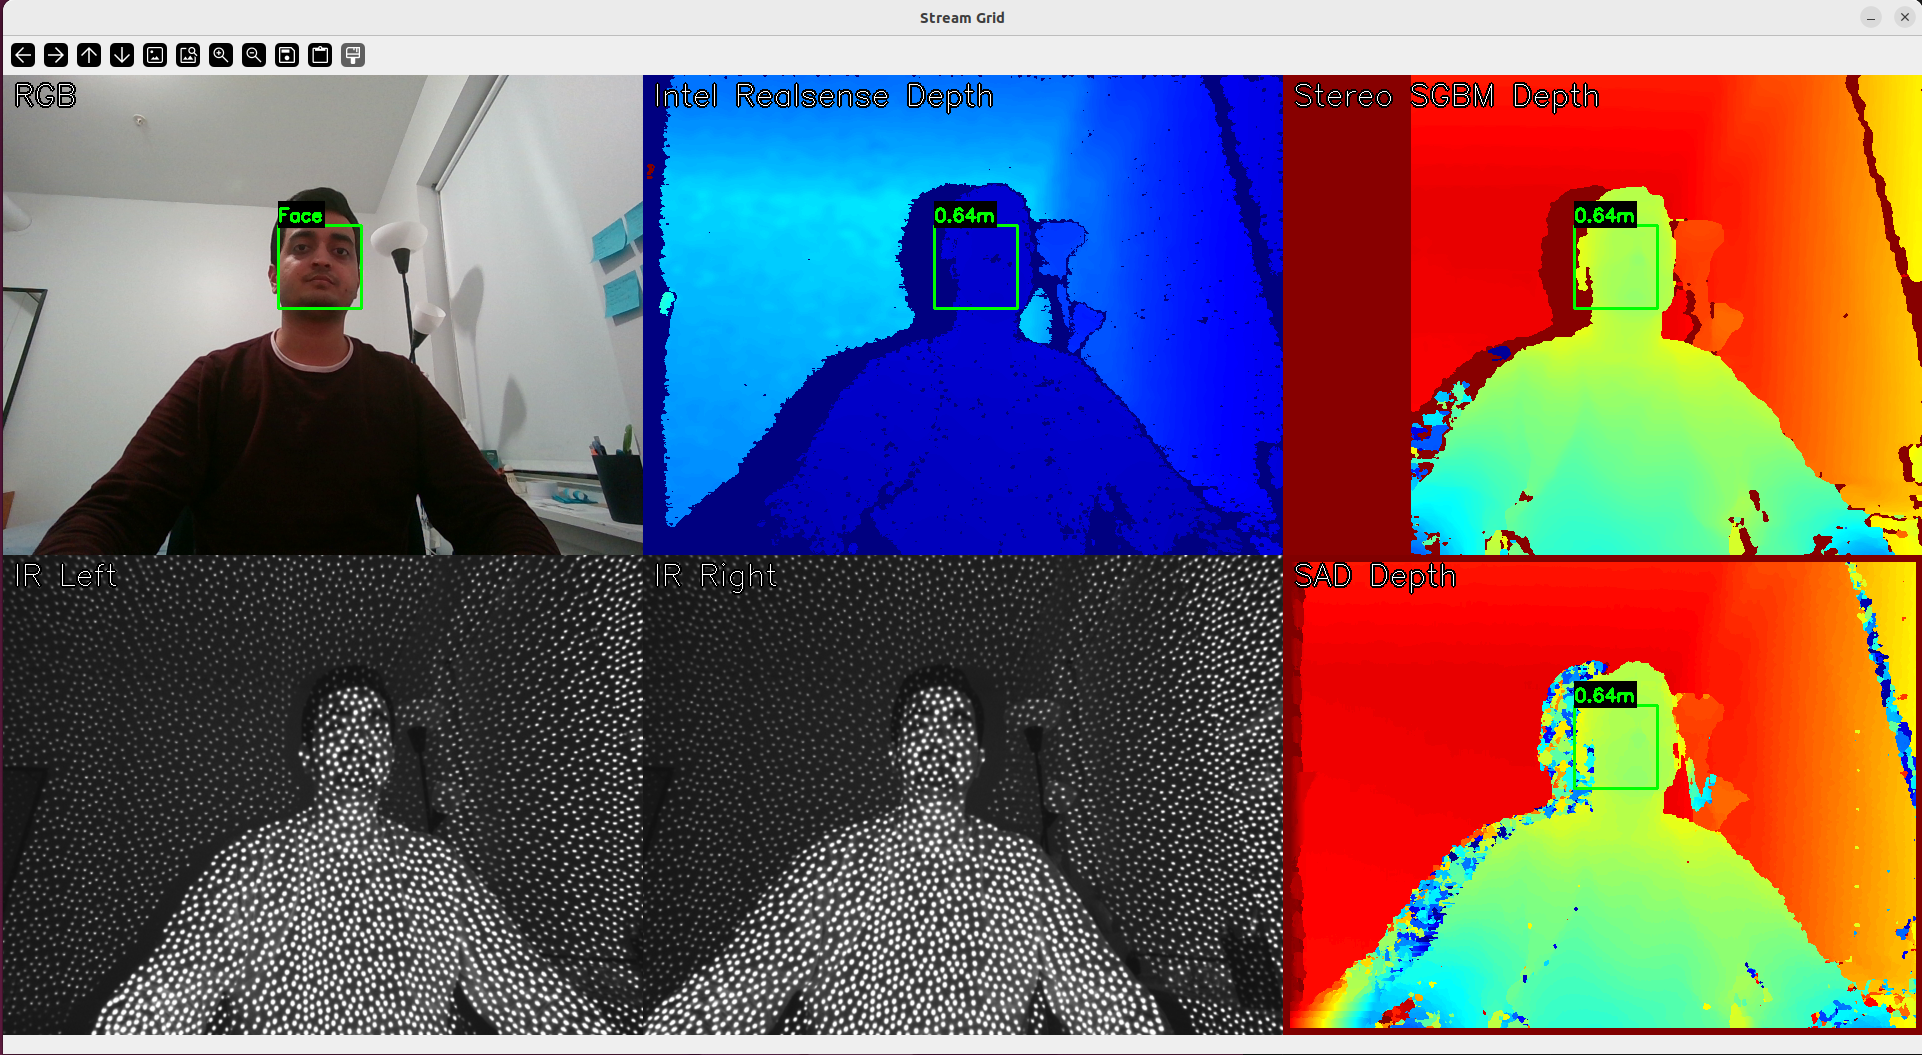
\includegraphics[width=\linewidth]{app_snap.png}
\caption{Live output of the running application. The six-panel grid shows (top
row, left to right): RGB with detected face and bounding box; Intel RealSense
hardware depth map reporting 0.64~m; OpenCV SGBM depth map reporting 0.64~m.
Bottom row: IR Left and IR Right streams showing the structured IR dot pattern
projected onto the scene; custom SAD depth map reporting 0.64~m. All three
depth methods agree on the face distance in this frame.}
\end{figure}

All three depth panels map depth to the \textbf{JET colourmap} such that
\textbf{near objects appear blue/cool} and \textbf{distant objects appear
red/warm}. In JET, low values map to blue and high values map to red.

The \textbf{hardware depth} panel achieves this naturally: Z16 depth values
increase with distance, so closer pixels produce smaller values and appear
blue:

\begin{lstlisting}[caption={Hardware depth colourmap --- direct JET mapping}]
# small depth = near = small value = blue; large depth = far = red
depth_color = cv2.applyColorMap(
    cv2.convertScaleAbs(depth_image, alpha=0.03), cv2.COLORMAP_JET)
\end{lstlisting}

The \textbf{SGBM and SAD} panels work in disparity space, where closer objects
have \emph{larger} disparity. To restore the same near-blue/far-red convention,
the disparity value is \textbf{inverted} (subtracted from 255) before applying
JET:

\begin{lstlisting}[caption={Inverted JET colourmap for disparity panels}]
# large disparity = near; after inversion: small value = blue (near)
display  = 255 - cv2.convertScaleAbs(disparity, alpha=255.0 / max_disparity)
colormap = cv2.applyColorMap(display, cv2.COLORMAP_JET)
\end{lstlisting}

Panel labels and depth readouts are drawn with a solid black background
rectangle to ensure readability over both dark and bright depth regions:

\begin{lstlisting}[caption={Text with background helper (live\_stream.py lines 35--40)}]
def put_text_with_bg(image, text, pos, font_scale, text_color, bg_color=(0,0,0)):
    font = cv2.FONT_HERSHEY_SIMPLEX
    (tw, th), baseline = cv2.getTextSize(text, font, font_scale, thickness=1)
    x, y = pos
    cv2.rectangle(image, (x, y-th-baseline), (x+tw, y+baseline), bg_color, cv2.FILLED)
    cv2.putText(image, text, pos, font, font_scale, text_color, thickness=1)
\end{lstlisting}

\newpage
% ─────────────────────────────────────────────────────────────────────────────
\section{Comparison of Approaches}
% ─────────────────────────────────────────────────────────────────────────────

\begin{center}
\begin{tabularx}{\linewidth}{lXXX}
  \toprule
  \textbf{Characteristic}   & \textbf{Hardware ASIC} & \textbf{OpenCV SGBM} & \textbf{Custom SAD} \\
  \midrule
  Algorithm       & Proprietary Intel firmware & Semi-global DP & Local block matching \\
  Block size      & Internal (unknown)  & 11$\times$11 px & 15$\times$15 px \\
  Search range    & Up to 1280 px       & 128 disparities & 128 disparities \\
  Global smoothing& Yes (temporal + spatial) & Yes (semi-global) & No \\
  Post-processing & Yes (many filters)  & Speckle + L-R check & None \\
  Sub-pixel acc.  & Yes (hardware)      & Yes ($\div 16$) & No (integer only) \\
  Noise level     & Very low            & Low--medium     & High (blocky) \\
  Edge quality    & Good                & Moderate        & Poor \\
  CPU compute     & N/A (on-device)     & $\sim$5--20 ms/frame & $\sim$100--500 ms/frame \\
  Code complexity & 1 SDK call          & $\sim$15 lines  & $\sim$40 lines \\
  \bottomrule
\end{tabularx}
\end{center}

\textbf{Key observations:}

\begin{itemize}
  \item \textbf{Hardware depth} is the most reliable. It benefits from temporal
        filtering, sub-pixel interpolation, and proprietary optimisation for
        the D455F sensor geometry.

  \item \textbf{SGBM} produces significantly smoother results than SAD. The
        dynamic programming smoothness penalties ($P_1$, $P_2$) discourage
        abrupt disparity changes, reducing noise. It is the best software
        alternative to hardware depth.

  \item \textbf{SAD} produces the noisiest depth maps. Without any global
        smoothness constraint, each pixel independently picks the best-matching
        disparity, leading to salt-and-pepper noise and incorrect matches in
        textureless regions. However, it is the most transparent algorithm for
        understanding the fundamentals of stereo matching.

  \item Despite the SAD implementation using the integral image trick for
        vectorised computation, iterating over 128 disparities sequentially
        in Python still makes it the slowest of the three methods.
\end{itemize}

\newpage
% ─────────────────────────────────────────────────────────────────────────────
\section{Dependencies and Libraries}
% ─────────────────────────────────────────────────────────────────────────────

\begin{center}
\begin{tabularx}{\linewidth}{llX}
  \toprule
  \textbf{Library} & \textbf{Version} & \textbf{Purpose and key APIs} \\
  \midrule
  \code{pyrealsense2} & 2.x &
    Camera control and frame capture. Key APIs: \code{rs.pipeline},
    \code{rs.config}, \code{enable\_stream}, \code{wait\_for\_frames},
    \code{get\_distance}, \code{get\_intrinsics}, \code{get\_extrinsics\_to}. \\[4pt]

  \code{OpenCV (cv2)} & 4.x &
    Stereo matching, visualisation, and image processing. Key APIs:
    \code{StereoSGBM\_create}, \code{compute}, \code{applyColorMap},
    \code{convertScaleAbs}, \code{cvtColor}, \code{rectangle}, \code{putText}. \\[4pt]

  \code{NumPy} & 2.x &
    Numerical array operations and the custom SAD implementation. Key APIs:
    \code{asanyarray}, \code{cumsum}, \code{full}, \code{zeros}, \code{abs},
    \code{hstack}, \code{vstack}, \code{astype}. \\[4pt]

  \code{MediaPipe} & 0.x &
    Deep learning inference for face detection. Key APIs:
    \code{tasks.vision.FaceDetector}, \code{FaceDetectorOptions},
    \code{mp.Image}, \code{detector.detect}. \\
  \bottomrule
\end{tabularx}
\end{center}

\begin{center}
\begin{tabular}{ll}
  \toprule
  \textbf{Model file property} & \textbf{Value} \\
  \midrule
  Filename          & \code{blaze\_face\_full\_range.tflite} \\
  Size              & $\approx$1.1~MB \\
  Format            & TensorFlow Lite (flatbuffer) \\
  Architecture      & BlazeFace (full-range variant) \\
  Detection range   & 20\%--100\% of image width \\
  Confidence threshold & 0.5 (configurable) \\
  Input format      & SRGB via \code{mp.Image} wrapper \\
  \bottomrule
\end{tabular}
\end{center}

% ─────────────────────────────────────────────────────────────────────────────
\section{How to Run}
% ─────────────────────────────────────────────────────────────────────────────

\subsection{Hardware Requirements}

\begin{itemize}
  \item \textbf{Intel RealSense D455F} camera connected via USB~3.1 Gen~1 or
        faster. USB~2 is not supported for multi-stream capture at 30~FPS.
  \item A machine with a CPU capable of running OpenCV SGBM and NumPy SAD in
        real time (any modern quad-core is sufficient, though SAD will be slow).
\end{itemize}

\subsection{System-Level Dependency: librealsense2}

\code{pyrealsense2} is a Python wrapper around Intel's \textbf{librealsense2}
C++ SDK, which must be installed at the OS level before the Python package will
work. On Ubuntu/Debian:

\begin{lstlisting}[language=sh, caption={Install librealsense2 SDK (Ubuntu)}]
# Register Intel's package server
sudo apt-key adv --keyserver keyserver.ubuntu.com \
     --recv-key F6E65AC044F831AC80A06380C8B3A55A6F3EFCDE
sudo add-apt-repository \
     "deb https://librealsense.intel.com/Debian/apt-repo $(lsb_release -cs) main"
sudo apt update

# Install SDK and utilities
sudo apt install -y librealsense2-dkms librealsense2-utils \
                    librealsense2-dev librealsense2-dbg
\end{lstlisting}

Verify the camera is detected before running the Python script:

\begin{lstlisting}[language=sh, caption={Verify camera connection}]
rs-enumerate-devices   # should list the D455F and its streams
\end{lstlisting}

\subsection{Python Environment Setup}

\begin{lstlisting}[language=sh, caption={Create environment and install dependencies}]
# Create and activate a virtual environment (recommended)
python3 -m venv .venv
source .venv/bin/activate          # Windows: .venv\Scripts\activate

# Install all Python dependencies
pip install -r requirements.txt
\end{lstlisting}

The \code{requirements.txt} pins the exact versions used during development:

\begin{center}
\begin{tabular}{ll}
  \toprule
  \textbf{Package} & \textbf{Version} \\
  \midrule
  \code{pyrealsense2}  & 2.56.5.9235 \\
  \code{numpy}         & 2.4.1 \\
  \code{opencv-python} & 4.13.0.92 \\
  \code{mediapipe}     & 0.10.33 \\
  \bottomrule
\end{tabular}
\end{center}

\subsection{Project File Checklist}

The following files must be present in the same directory before running:

\begin{center}
\begin{tabular}{lll}
  \toprule
  \textbf{File} & \textbf{Required} & \textbf{Notes} \\
  \midrule
  \code{live\_stream.py}                  & Yes & Main application script \\
  \code{blaze\_face\_full\_range.tflite}  & Yes & BlazeFace model; must be in the working directory \\
  \code{requirements.txt}                 & Yes & Python dependency list \\
  \bottomrule
\end{tabular}
\end{center}

\subsection{Running the Application}

With the camera connected and the environment active, run:

\begin{lstlisting}[language=sh, caption={Launch the live stream}]
python3 live_stream.py
\end{lstlisting}

A window titled \textbf{Stream Grid} will open displaying the $2 \times 3$
panel layout. Press \textbf{Q} or close the window to stop the application
cleanly --- the \code{finally} block in the script ensures
\code{pipeline.stop()} is always called, releasing the camera.

\begin{notebox}
\textbf{Expected startup time:} The first frame takes 1--3 seconds to appear
while the camera pipeline initialises and the BlazeFace model is loaded into
memory. The SAD depth panel will update noticeably slower than the other panels
due to its sequential per-disparity computation over 128 levels.
\end{notebox}

\subsection{Common Issues}

\begin{center}
\begin{tabularx}{\linewidth}{lX}
  \toprule
  \textbf{Error} & \textbf{Fix} \\
  \midrule
  \code{RuntimeError: No device connected} &
    Check USB cable and port (must be USB~3). Run \code{rs-enumerate-devices}
    to confirm the camera is visible to the SDK. \\[4pt]
  \code{Failed to load model} &
    Ensure \code{blaze\_face\_full\_range.tflite} is in the same directory as
    \code{live\_stream.py}, or provide an absolute path. \\[4pt]
  \code{cv2.error: (-215) disparity} &
    IR frames must be grayscale (Y8). Confirm stream format is
    \code{rs.format.y8} in the config. \\[4pt]
  Blank / black depth panels &
    The IR dot projector may be disabled. Use \code{realsense-viewer} to
    confirm both IR streams are active and the projector is on. \\
  \bottomrule
\end{tabularx}
\end{center}

% ─────────────────────────────────────────────────────────────────────────────
\section{Conclusion}
% ─────────────────────────────────────────────────────────────────────────────

This project demonstrates a complete real-time stereo vision pipeline for face
depth estimation using the Intel RealSense D455F. Three independently
implemented depth methods operate in parallel on the same hardware streams,
providing a direct comparison of their characteristics.

\begin{itemize}
  \item \textbf{Hardware ASIC depth} provides the best quality with the least
        code. It leverages Intel's proprietary stereo processor and requires
        only a single SDK call. It is the practical solution for real-world
        applications.

  \item \textbf{OpenCV SGBM} demonstrates how a classical computer vision
        algorithm can approach hardware-quality depth by incorporating global
        smoothness constraints through semi-global dynamic programming.

  \item \textbf{Custom SAD block matching} provides the clearest educational
        view of how stereo matching works at the fundamental level. Despite
        being the simplest and noisiest method, it illuminates the core
        principle behind all stereo vision: finding corresponding pixels across
        two viewpoints and measuring their horizontal displacement.
\end{itemize}

The integration of BlazeFace for lightweight real-time face detection, combined
with the vectorised NumPy implementation of SAD (using the cumulative sum
trick), illustrates how modern deep learning tools and classical optimisation
techniques can coexist effectively in a single real-time system.

\begin{notebox}
\textbf{Possible extensions:} applying WLS (Weighted Least Squares)
post-filtering on SGBM disparities to reduce noise near edges; implementing
temporal depth smoothing for face tracking; benchmarking all three methods
against a known ground-truth distance; or replacing the SAD matching cost with
the more robust Census transform.
\end{notebox}

\end{document}
